\section{Introduction}
\label{sec:intro}

Topic models explain document collections at a high
level~\cite{boyd-graber-2017-topic-model-book}.
%
Multilingual topic models (\mtms) uncover latent topics \emph{across}
languages and reveal
%The latent topics---represented as distributions over
%words---summarize documents and help analysts discover trends~\cite{lau-2012-tm-trend}, analyze
%emotions~\cite{bao-2009-tm-emotions}, or recommend content~\cite{marlin-2003-tm-cf}.\jbgcomment{Add some monolingual
%  citations here, perhaps changing the applications.}\wycomment{Done.}
%In contrast to monolingual topic models, \mtms reveal
commonalities and differences across languages
and cultures~\cite{ni-2009-mtm-wiki,shi-2016-mtm-common,gutierrez-2016-mtm-diff}.
Existing models extend latent Dirichlet
allocation~\cite[\lda]{blei-2003-lda} and learn \emph{aligned} topics
across languages~\cite{mimno-2009-plda}.

Prior models work well because they implicitly assume---even if not part of the
model---parallel or highly comparable data with well-aligned topics.
%
However, this
assumption does not always comport with reality.
%
Even documents from the same place and time
can discuss very different things across languages: in multicultural
London, Hindi tweets focus on a Bollywood actor's
\abr{bbc} appearance, French blogs fret
about Brexit, and English articles focus on Tottenham's lineup.
%
Generally, corpora have a range of ``nonparallelness''~\citep{fung-2000-bilingual-stat}.
%
In less comparable settings,
% Even in a ``comparable'' setting,
%consideration of multiple languages brings to the forefront the fact that,
while some topics are shared, languages' emphasis may diverge
and some topics may lack analogs.

% Unfortunately, it is not always the case that the cross-lingual
% documents are highly comparable or parallel. Even on the same topic,
% the documents in different languages may talk about different
% aspects. For instance, in the news articles about
% \underline{Earthquake}, we find that the English articles talk about
% the worldwide earthquakes, while the Chinese articles focus on the
% earthquake happened in Sichuan Province in 2008. Such difference in
% topics and topic aspects can fail a \mtm which aligns all topics,
% because they do not let people know which topics are shared across
% languages and which are unique in a language.


\begin{figure}[t]
  \centering
  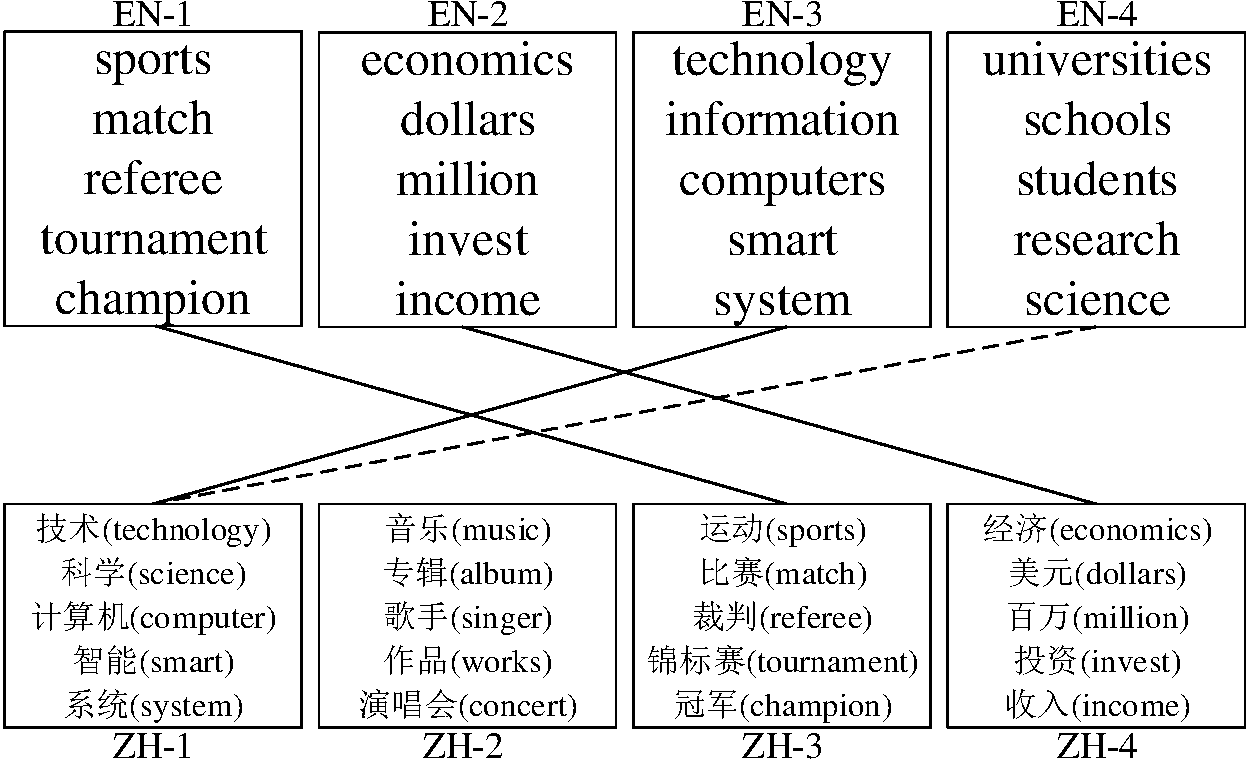
\includegraphics[width=.96\linewidth]{2019_emnlp_mtm/figures/topic_link_vertical2.pdf}
  \caption{\ignore{Our \mtm learns weighted topic links: }Topic pairs
    with many word translation pairs have high link weights, e.g.,
    (\en-1, \zh-3) and (\en-2, \zh-4); topic pairs with partial
    overlap receive lower weights, e.g., (\en-4, \zh-1); a topic is
    unlinked if there is no corresponding topic in the other language
    (\zh-2).\jbgcomment{We're not using the full width of the figure, and the Hanzi are very skinny; try to use the width to at least get a topic label in for the Chinese topics.  Otherwise it's not very useful to someone who doesn't speak Chinese\wycomment{Done.}}
  }\label{fig:topic_link_example}
\end{figure}


We therefore introduce a new multilingual topic model that assumes
each language has its own topic sets and jointly learns all topics,
but does not force one-to-one alignment across languages.
%
Instead, our \mtm learns \emph{weighted} topic links across languages
and only assigns a high link weight to a topic pair whose top words
have many direct translation pairs
(Figure~\ref{fig:topic_link_example}).
%, so they are weakly linked, while \zh-1 is strongly linked with \en-4.
Moreover, it allows unlinked topics if there is no matching topic in
the other language. This makes the model robust for (more common)
less-comparable data with topic misalignment.
%
Joint inference also allows insights from
high-resource languages to uncover low-resource language patterns. It is particularly useful
in scenarios that involve modeling topics on low-resource languages in humanitarian assistance, peacekeeping,
and/or infectious disease response, while limiting the additional cost to other steps that will also need to be taken,
such as finding or creating a word translation dictionary.

\psrnewcomment{Reference to humanitarian assistance felt out of
  place. \jbgcomment{Would be good to add back in now that we have
    more space, connect better to LORELEI.} \wycomment{Done.}}

% We describe our \mtm in the bilingual case which has a language~$S$ with $K_S$ topics and another language~$T$ with $K_T$ topics, and it is fairly easy to generalize it to multilingual. The \mtm has two matrices~\rhots and~\rhost that store topic link weight matrices and convert the topics from language~$T$ to~$S$ and~$S$ to~$T$ respectively. For a translation pair, its two words have the same sense, so the topics in which the two words are assigned high probability mass are likely to be corresponding topics of each other in the two languages. Therefore, the values of~$\bm{\rho}$'s are learned through converting the words' topic distributions in one language into the topic space of the other language using~$\bm{\rho}$'s and making them as close as possible to their translation words' topic distributions in the other language (see Section~\ref{sec:model}). In this process, the shared topic pairs across languages will get higher weights, while a unique topic in a language will have a high-entropy weight distribution over the topics in the other language.

We validate the \mtm in two classification tasks using
inferred topic posteriors as features.
%
Our \mtm has higher F1 than other models in both intra- and
cross-lingual evaluations, while discovering coherent topics and
meaningful topic links.
